% Sample homework assignment template with examples
% Copyright (C) April 2012 Joseph Paul Cohen (used style to create umb template)
%
% Basic LaTeX Template for Homework Submission with Formal Title Page
% Copyright (C) 2012 Patrick McLaren
%
%
% This program is free software: you can redistribute it and/or modify
% it under the terms of the GNU General Public License as published by
% the Free Software Foundation, either version 3 of the License, or
% (at your option) any later version.
%
% This program is distributed in the hope that it will be useful,
% but WITHOUT ANY WARRANTY; without even the implied warranty of
% MERCHANTABILITY or FITNESS FOR A PARTICULAR PURPOSE.  See the
% GNU General Public License for more details.
%
% You should have received a copy of the GNU General Public License
% along with this program.  If not, see <http://www.gnu.org/licenses/>.


% Author Info
\def\thetitle{Title}
\def\theauthor{Firstname Lastname}
\def\email{email@cs.umb.edu}
\def\theclass{CS999}
\def\studentid{Student ID\#}
\def\thedate{\today}
\def\university{University of Massachusetts Boston}

%%%%%%%%%%%%%%%%%%%%%%%%%%%%%%%%%%%%%%%%%
%%%%%%%%%%%%%%%%%%%%%%%%%%%%%%%%%%%%%%%%%
%% You can ignore all this stuff for now
%%%%%%%%%%%%%%%%%%%%%%%%%%%%%%%%%%%%%%%%%

\documentclass[12pt,letterpaper]{article}

\usepackage{amsmath,amsfonts,amsthm,amssymb}
\usepackage{setspace}
\usepackage{Tabbing}
\usepackage{lastpage}
\usepackage{extramarks}
\usepackage{chngpage}
\usepackage{soul,color}
\usepackage{graphicx,float,wrapfig}
\usepackage[ruled,vlined,linesnumbered]{algorithm2e}
\usepackage{url}

%Tikz
\usepackage{tikz}
\usetikzlibrary{trees,snakes}
\usetikzlibrary{arrows,automata}
\usetikzlibrary{matrix}
\usetikzlibrary{calc}

\setlength{\parskip}{0pt} % 1ex plus 0.5ex minus 0.2ex}
\setlength{\parindent}{0pt}

% Increase to 2.0 for double spacing.
\linespread{1}

% Header & Footers
% LaTeX has very generous margins, by default.
% I've shrunk the margins, considerably.
\usepackage[hmargin=2cm,vmargin=3.5cm]{geometry}
\usepackage{fancyhdr}
\pagestyle{fancy}
\lhead{\thetitle}
\chead{}
\rhead{\theauthor}
\lfoot{}
\cfoot{\theclass\ - \thedate}
\rfoot{\thepage}
\renewcommand{\headrulewidth}{0.5pt}
\renewcommand{\footrulewidth}{0.5pt}

\begin{document}

% Title Page
\begin{titlepage}
\begin{center}
\textsc{\LARGE \university}\vspace{10mm}
\hrule\vspace{2mm}
\huge\bfseries\thetitle\vspace{2mm}
\hrule\vspace{10mm}
\end{center}
\begin{flushleft}
\textbf\theauthor\\
\studentid\\
\email\\
\end{flushleft}
\vfill
\begin{center}
\thedate
\end{center}
\end{titlepage}
\newpage


%%%%%%%%%%%%%%%%%%%%%%%%%%%%%%%%%%%%%%%%%
%%%%%%%%%%%%%%%%%%%%%%%%%%%%%%%%%%%%%%%%%
%%%%%%%%%%%%%%%%%%%%%%%%%%%%%%%%%%%%%%%%%
%%%%%%%%%%%%%%%%%%%%%%%%%%%%%%%%%%%%%%%%%
%% You work below this part
%%%%%%%%%%%%%%%%%%%%%%%%%%%%%%%%%%%%%%%%%

\section*{Problem 1}

Why should you use this template?

\begin{enumerate}
  \item Latex makes it easy to have great looking homeworks
  \item \LaTeX ``tex'' files work great with revision control systems such as
  $svn$ and $git$
  \item Math is much easier to write $\displaystyle\sum_{i=0}^\infty
  i(1-p^+)^{i-1}p^+ = \frac{p^+}{(1-(1-p^+))^2}$
  \item Can can store all your old homeworks without scanning them
  \item You will know the name of all the symbols you use
  \item Professors will spend less time trying to figure out your handwriting
  \item If you do your homework in \LaTeX during your undergrad, you can spend
  more time researching as a graduate student.
\end{enumerate}

\section*{Problem 1.1}

\begin{itemize}
  \item Lorem ipsum dolor sit amet, consectetur adipiscing elit. Aenean et
  condimentum nunc. Nulla a mattis quam. Nullam vitae eros dui, sit amet
  fringilla quam. Nulla facilisi. Nulla aliquam ipsum eget turpis porttitor
  luctus. Proin sem ante, $\sum_{i=0}^\infty
  i(1-p^+)^{i-1}p^+ = \frac{p^+}{(1-(1-p^+))^2}$ lobortis nec euismod id,
  imperdiet quis eros. Donec sit amet diam at leo pretium dignissim. Donec molestie velit eget orci
  adipiscing euismod ut sit amet lorem. Pellentesque elementum faucibus diam sit
  amet aliquam. Nullam augue massa, ullamcorper vel rhoncus sit amet, posuere ac
  mauris. Nulla commodo dapibus leo quis condimentum.
  \item \begin{enumerate}
    \item Lorem ipsum dolor sit amet, consectetur adipiscing
	elit.  Aenean et condimentum nunc. Nulla a mattis quam. Nullam vitae eros dui,
	sit amet fringilla quam. 
	\item Nulla facilisi. Nulla aliquam ipsum eget turpis
	porttitor luctus. Proin sem ante, lobortis nec euismod id, imperdiet quis eros.
	Donec sit amet diam at leo pretium dignissim. 
	\item Donec molestie velit eget orci
	adipiscing euismod ut sit amet lorem. Pellentesque elementum faucibus diam sit
	amet aliquam. 
	\item Nullam augue massa, ullamcorper vel rhoncus sit amet, posuere ac
	mauris. Nulla commodo dapibus leo quis condimentum.
  \end{enumerate}
\end{itemize}

Sometimes we want a fixed width font:

\begin{verbatim}
#!/bin/bash          
tar -cZf /var/my-backup.tgz /home/me/
echo Hello World   
\end{verbatim}


\newpage
\section*{Problem 2}

You want to include images? Check out Figures \ref{fig:umblogo} and
\ref{fig:3umblogo}.

\begin{figure}[h]
\begin{center}

\includegraphics[width=.2\textwidth]{umass-boston-logo.png}
\caption{The UMASS Boston Logo}
\label{fig:umblogo}
\end{center}
\end{figure} 

\begin{figure}[h]
\begin{center}

\includegraphics[width=.2\textwidth]{umass-boston-logo.png}

\includegraphics[width=.2\textwidth]{umass-boston-logo.png}

\includegraphics[width=.2\textwidth]{umass-boston-logo.png}
\caption{The UMASS Boston Logo}
\label{fig:3umblogo}
\end{center}
\end{figure} 

\newpage
\section*{Problem 3}

You want to draw a tree?  You can use the Tikz library. This library is amazing.
You can check out examples here at \url{http://www.texample.net/tikz/}


\begin{center}
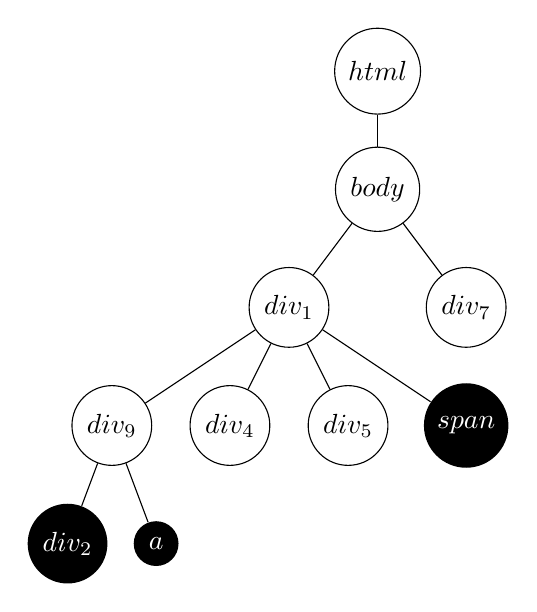
\begin{tikzpicture}[
level/.style={sibling distance=60mm/#1},
leaf/.style={circle, draw=none, fill=black,
        text centered, text=white}
]

\begin{scope}[level/.style={sibling distance=45mm/#1}]
\node [circle,draw] (z){$html$}

% <body>
child {node [circle,draw] (body) {$body$}
% 	<div id="1">
	child {node [circle,draw] (1) {$div_1$}
% 		<div id="9">
		child {node [circle,draw] (9) {$div_9$}
% 			<div id="2">div2</div>
			child {node [circle,draw,leaf] (2) {$div_2$}}
% 			<a> a </a>
			child {node [circle,draw,leaf] (a) {$a$}}
		}
% 		</div>
% 		<div id="4"></div>
		child {node [circle,draw] (4) {$div_4$}	
	}
% 	</div>
% 		<div id="5">
		child {node [circle,draw] (5) {$div_5$}}
% 			<span id="6">span</span>
			child {node [circle,draw,leaf] (span) {$span$}}
		}
% 		</div>
% 	<div id="7"></div>
	child {node [circle,draw] (7) {$div_7$}}
};
% </body> 

\end{scope}
\end{tikzpicture}
\end{center}



\begin{center}
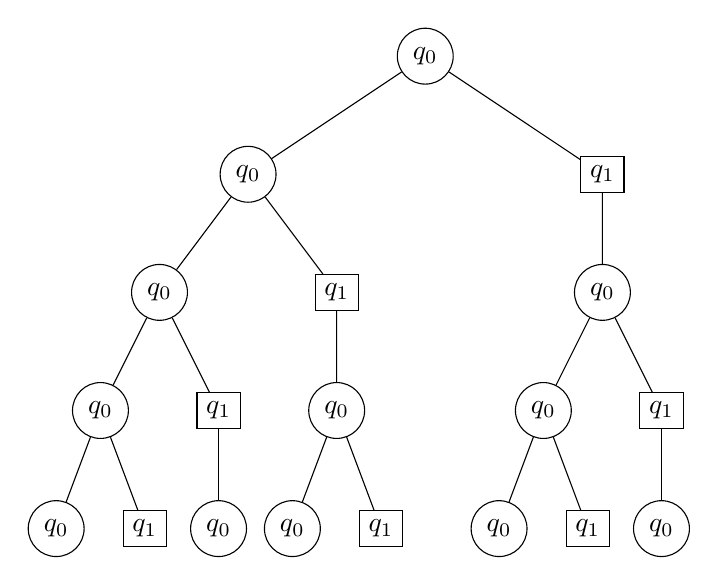
\begin{tikzpicture}[
	level/.style={sibling distance=45mm/#1},
	leaf/.style={circle, draw=none, fill=black,
	        text centered, text=white}
	]
	\node [circle,draw] (z){$q_0$}
	
	child {node [circle,draw] {$q_0$}
			child {node [circle,draw] {$q_0$}
			child {node [circle,draw] {$q_0$}
				child {node [circle,draw] {$q_0$}}
				child {node [draw] {$q_1$}}
				}
			child {node [draw] {$q_1$}
				child {node [circle,draw] {$q_0$}}
				}
			}
		child {node [draw] {$q_1$}
			child {node [circle,draw] {$q_0$}
			child {node [circle,draw] {$q_0$}}
			child {node [draw] {$q_1$}}
		}
	}
	}
	child {node [draw] {$q_1$}
		child {node [circle,draw] {$q_0$}
		child {node [circle,draw] {$q_0$}
			child {node [circle,draw] {$q_0$}}
			child {node [draw] {$q_1$}}
		}
		child {node [draw] {$q_1$}
			child {node [circle,draw] {$q_0$}}
			}
	}
	}
	;
\end{tikzpicture}
\end{center}


\subsection*{Automata}




\begin{center}
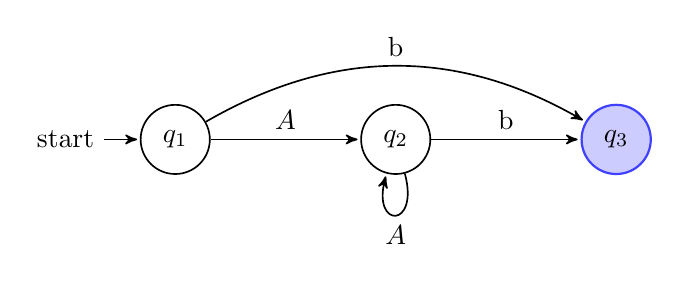
\begin{tikzpicture}[->,>=stealth',shorten >=1pt,auto,node
distance=2.8cm,semithick] 
  \tikzstyle{final}=[circle,thick,draw=blue!75,fill=blue!20,text=black] 
  \node[initial,state] 	(1)                    	{$q_1$}; 
  \node[state]   		(2) [right of=1] 	  	{$q_2$};
  \node[state, final]   (3) [right of=2] 	  	{$q_3$};
	
  \path (1) edge [bend left] 	node {b} (3)
            edge              	node {$A$} (2)
        (2) edge  		      	node {b} (3)
        	edge [loop below] 	node {$A$} (2)
        ;
\end{tikzpicture}
\end{center}






\begin{center}
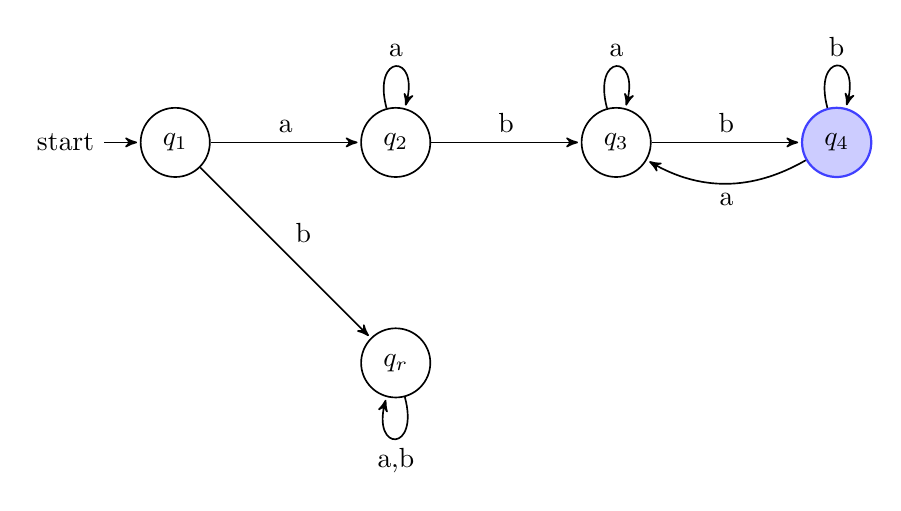
\begin{tikzpicture}[->,>=stealth',shorten >=1pt,auto,node distance=2.8cm,semithick]
	  \tikzstyle{every state}=[text=black]
	  \tikzstyle{final}=[circle,thick,draw=blue!75,fill=blue!20,text=black] 
	  \node[initial,state] (1)                    {$q_1$}; 
	  \node[state]         (2) [right of=1] 	  {$q_2$};
	  \node[state]  (3) [right of=2] 	  {$q_3$};
	  \node[state, final]  (4) [right of=3] 	  {$q_4$};
	  \node[state]         (r) [below of=2] 	  {$q_r$};
		
	  \path (1) edge              node {a} (2) 
	            edge              node {b} (r)
	        (2) edge [loop above] node {a} (2)
	            edge              node {b} (3)
	        (3) edge [loop above] node {a} (3)
	        	edge              node {b} (4)
	        (4) edge [bend left]  node {a} (3)
	        	edge [loop above] node {b} (3)
	        (r) edge [loop below] node {a,b} (4);
\end{tikzpicture}
\end{center}









\begin{center}

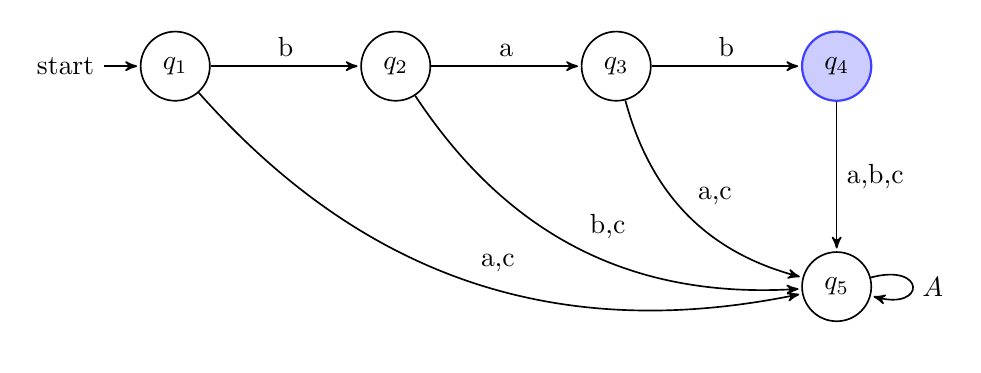
\begin{tikzpicture}[->,>=stealth',shorten >=1pt,auto,node
		distance=2.8cm,semithick] 
  \tikzstyle{final}=[circle,thick,draw=blue!75,fill=blue!20,text=black] 
  \node[initial,state] 	(1)                    	{$q_1$}; 
  \node[state]         	(2) [right of=1] 	  	{$q_2$};
  \node[state]         	(3) [right of=2] 	  	{$q_3$};
  \node[state, final]   (4) [right of=3] 	  	{$q_4$};
  \node[state]  		(5) [below of=4]       	{$q_5$};
	
  \path (1) edge [bend right] node {a,c} (5)
            edge              node {b} (2)
        (2) edge  		      node {a} (3)
        	edge [bend right] node {b,c} (5)
        (3) edge 			  node {b} (4)
        	edge [bend right] node {a,c} (5)
        (4) edge              node {a,b,c} (5)
        (5)	edge [loop right] node {$A$} (5);
\end{tikzpicture}

\end{center}








\newpage
\section*{Problem 4}

You want to do some linear algebra?

$$V = \left(\begin{array}{c c c}
v_{1,1} & \ldots & v_{1,n}\\
\vdots & \ddots\\
v_{2,1} & \ldots & v_{2,n}\\
\vdots & \ddots\\
v_{m,1} & \ldots & v_{m,n}\\
\end{array}
\right)$$

$$\underbrace{rank(AB)}_n 
= \underbrace{rank(B)}_{\leq n}
-dim(\underbrace{null(A)}_0\cap \underbrace{range(B)}_n)$$

\begin{equation}
M_f = \left(\begin{array}{l l l}
a & b\\
c & d\\
\end{array}
\right) $$

$$M_f M_g = \left(\begin{array}{l l l}
ae+bg & af+bh\\
ce+dg & cf+dh\\
\end{array}
\right)
\end{equation}


$$\displaystyle\sum_{i=1}^n \displaystyle\sum_{j=1}^n b_{ij} = 0$$


$$\left\{\begin{array}{l l l}
y_1u_{1,1} + y_2u_{1,2},\ldots,y_n u_{1,n} = 0\\
y_1u_{2,1} + y_2u_{2,2},\ldots,y_n u_{2,n} = 0\\
\ldots \\
y_1u_{m,1} + y_2u_{m,2},\ldots,y_n u_{m,n}  = 0\\
\end{array}
\right. $$

\newpage
\section*{Problem 5}

So you want to write an algorithm?

\begin{algorithm}[h]
\caption{\label{alg:sta}Simple Tree Matching}
\KwIn{Tree $a$ \\
\hspace{42pt}Tree $b$}
\KwOut{Integer $match$}

\If{a and b contain distinct symbols}{

return $0$

}\Else{

$m \leftarrow $ the number of first-level sub-trees of $a$

$n \leftarrow $ the number of first-level sub-trees of $b$

$M[i,0] \leftarrow 0 $ for $ i = 0,\ldots,m$

$M[0,j] \leftarrow 0 $ for $ j = 0,\ldots,n$

\For{$i = 1$ to $m$}{
	
	\For {$i = 1$ to $n$}{
		
		$x \leftarrow M[i,j-1]$
		
		$y \leftarrow M[i-1,j]$
		
		$z \leftarrow M[i-1,j-1]+ SimpleTreeMatch(a_i,b_j)$
		
		$M[i,j]	\leftarrow max(x,y,z)$
	}
}
return $M[m,n] + 1$
}

\end{algorithm}

\newpage
\section*{Problem 6}

Want to make tables?

\begin{center}
    \begin{tabular}{ | c | c | c |}
    \hline
    Set & $a^{-1}(Set)$ & $b^{-1}(Set)$ \\ 
    \hline 
    \hline
    $aA^*bA^*b$ & $A^*bA^*b \cup bA^*b$ & $\emptyset$ \\ 
    \hline
    $A^*bA^*b \cup bA^*b$ & $A^*bA^*b \cup bA^*b$ & $A^*bA^*b \cup bA^*b \cup
    A^*b \cup b$ \\ 
    \hline 
    $A^*bA^*b \cup bA^*b \cup A^*b \cup b$ & 
    $A^*bA^*b \cup bA^*b \cup A^*b \cup b$ &
    $A^*bA^*b \cup bA^*b \cup A^*b \cup b \cup \lambda$ \\
    \hline 
    $A^*bA^*b \cup bA^*b \cup A^*b \cup b \cup \lambda$ & 
    $A^*bA^*b \cup bA^*b \cup A^*b \cup b$ &
    $A^*bA^*b \cup bA^*b \cup A^*b \cup b \cup \lambda$ \\
    
    \hline
    \end{tabular}
\end{center}




\begin{center}


\begin{tabular}{c|cc}
		$\Delta$ & 0 & 1\\
		\hline
		$q_0$ & $q_1$ & $q_1$\\ 
		\hline
		$q_1$ & $q_1$ & $q_1$\\ 
\end{tabular}

\end{center}





\begin{center}
\begin{tabular}{c|c|c|c|c}
Name & Lang & Clean & Rep. & Query\\
\hline
JSoup & Java & $\star$ & $\star$ & $\star$\\
\hline
NokoGiri & Ruby & $\star$ & $\star$ & $\star$\\
\hline
TagSoup & Java & $\star$ & $\star$ & $\star$\\
\hline
Taggle & C++ & $\star$ & $\star$ & $\star$\\
\hline
Rubyful Soup
\footnote{\url{http://www.crummy.com/software/RubyfulSoup/}} & Ruby
&$\star$ & $\star$ & $\star$\\
\hline
Beautiful Soup \footnote{\url{http://www.crummy.com/software/BeautifulSoup/}}
&Python&$\star$ & $\star$ & $\star$\\
\hline
NekoHtml \footnote{http://nekohtml.sourceforge.net/}  & Java & $\star$ & $\star$&$\star$\\
\hline
Xom  \footnote{http://www.xom.nu/} & Java & & $\star$ & $\star$\\
\hline
Saxon \footnote{http://saxon.sourceforge.net/} & Java & & $\star$ &$\star$\\
\hline
Xerces \footnote{http://xerces.apache.org/}& Java & & $\star$ &$\star$\\
\hline
HTMLParser \footnote{http://htmlparser.sourceforge.net/} & Java & & $\star$&$\star$\\
\hline
XStream \footnote{http://xstream.codehaus.org/} & Java & & $\star$&$\star$\\
\hline
Dom4j \footnote{http://dom4j.sourceforge.net/} & Java & & $\star$ & $\star$\\
\hline
HTML Tidy \footnote{http://tidy.sourceforge.net/} & C & $\star$ & &\\
\hline
JTidy \footnote{http://jtidy.sourceforge.net/} & Java & $\star$ & &\\
\hline
Tika \footnote{http://tika.apache.org/} & Java & $\star$ & &\\
\hline
HTMLCleaner \footnote{http://htmlcleaner.sourceforge.net/} & Java & $\star$ & &\\
\hline
Jaxen \footnote{http://jaxen.codehaus.org/} & Java & & &$\star$\\
\hline
Xalan \footnote{http://xml.apache.org/xalan-j/} & Java & & &$\star$\\
\hline

\end{tabular}
\end{center}



\newpage

\section*{Problem 7}

Sometimes we want to do things for a math class:
\begin{center}
\begin{tikzpicture}
  \matrix (m) [matrix of math nodes, row sep=3em,
    column sep=3em]{
    & f^\ast E_V& & \vphantom{f^\ast}E_V \\
    f^\ast E & & \vphantom{f^\ast}E & \\
    & U & & V \\
    M & & N & \\};
  \path[-stealth]
    (m-1-2) edge (m-1-4) edge (m-2-1)
            edge [densely dotted] (m-3-2)
    (m-1-4) edge (m-3-4) edge (m-2-3)
    (m-2-1) edge [-,line width=6pt,draw=white] (m-2-3)
            edge (m-2-3) edge (m-4-1)
    (m-3-2) edge [densely dotted] (m-3-4)
            edge [densely dotted] (m-4-1)
    (m-4-1) edge (m-4-3)
    (m-3-4) edge (m-4-3)
    (m-2-3) edge [-,line width=6pt,draw=white] (m-4-3)
            edge (m-4-3);
\end{tikzpicture}
\end{center}



\begin{center}


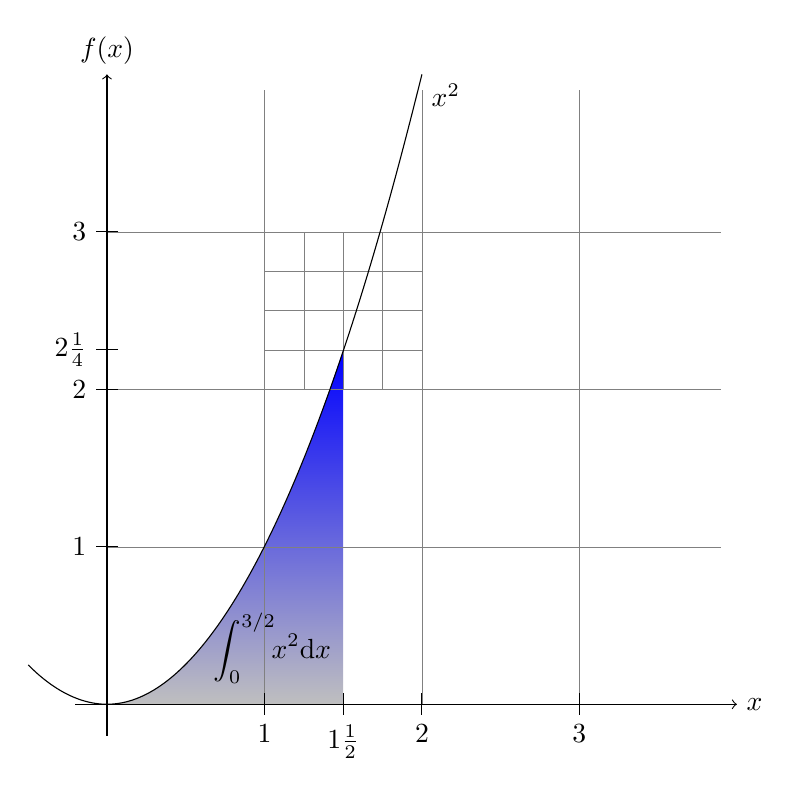
\begin{tikzpicture}[scale=2]
  \shade[top color=blue,bottom color=gray!50] 
      (0,0) parabola (1.5,2.25) |- (0,0);
  \draw (1.05cm,2pt) node[above] 
      {$\displaystyle\int_0^{3/2} \!\!x^2\mathrm{d}x$};

  \draw[style=help lines] (0,0) grid (3.9,3.9)
       [step=0.25cm]      (1,2) grid +(1,1);

  \draw[->] (-0.2,0) -- (4,0) node[right] {$x$};
  \draw[->] (0,-0.2) -- (0,4) node[above] {$f(x)$};

  \foreach \x/\xtext in {1/1, 1.5/1\frac{1}{2}, 2/2, 3/3}
    \draw[shift={(\x,0)}] (0pt,2pt) -- (0pt,-2pt) node[below] {$\xtext$};

  \foreach \y/\ytext in {1/1, 2/2, 2.25/2\frac{1}{4}, 3/3}
    \draw[shift={(0,\y)}] (2pt,0pt) -- (-2pt,0pt) node[left] {$\ytext$};

  \draw (-.5,.25) parabola bend (0,0) (2,4) node[below right] {$x^2$};
\end{tikzpicture}


\end{center}


\end{document}